\chapter{B-splines, NURBS and B\acuteacc ezier Curves}%
\label{SEC:SPLINES-APPENDIX}
This appendix briefly collects the central notions and properties of B-Splines, NURBS, and
B\acuteacc ezier curves, borrowing the formalism and the framework from~\cite{biagiotti2008trajectory}.
We start with a general overview of the three curve parameterizations mentioned above,
then go deep through their properties and correlations.
For further details, the reader is referred to~\cite{biagiotti2008trajectory, qin1998general, farouki2012bernstein}.

%----------------------------------------------------------------------------------------
\section{B-Spline Curves}
A \emph{B-spline}, or \emph{Basic-spline}, is a computationally efficient technique to implement
interpolating splines or to approximate functions, curves, and surfaces.
Any generic spline can be expressed in \emph{B-form} by linearly combining a proper
number of B-splines basis functions $\basis_i^{\order} \lp \splinevar \rp$,
\begin{equation*}
    \begin{matrix}
        \bs{\spline} \lp \splinevar \rp = \sum_{i=0}^{\cpnumber} \bs{\cpoint}_i \basis_i^{\order} \lp \splinevar \rp &
        \text{with} & \splinevar_{\text{min}} \le \splinevar \le \splinevar_{\text{max}},
    \end{matrix}
\end{equation*}
where $\order$ is the curve order, while the coefficients $\bs{\cpoint}_i \in \R^{n}$, $i = 0, \dots, \cpnumber$, are known
as \emph{control points} and can be computed by imposing some approximation or interpolation conditions on
a given set of data points. Let $\bs{\splinevar} = \lps \splinevar_0, \dots, \splinevar_{\order + \cpnumber + 1} \rps$
be a nondecreasing vector of real numbers, in this framework called \emph{knots}, then the $j$th B-spline
basis function of order $\order$ can be recursively computed via the De-Boor formula~\cite*{de1978practical}
\begin{equation*}
    \begin{split}
        \basis_i^0 \lp \splinevar \rp & =
        \begin{cases}
            \begin{matrix}
                1 & \text{if} & \splinevar_i \le \splinevar < \splinevar_{i+1},
            \end{matrix} \\
            \begin{matrix}
                0 & \text{otherwise},
            \end{matrix} \\
        \end{cases} \\
        \basis_i^{\order} \lp \splinevar \rp & = \frac{\splinevar - \splinevar_i}{\splinevar_{i+\order} - \splinevar_i}
        \basis_{i}^{\order-1} \lp \splinevar \rp
        + \frac{\splinevar_{i+\order+1} - \splinevar}{\splinevar_{i+\order+1} - \splinevar_{i+1}} \basis_{i+1}^{\order-1} \lp \splinevar \rp.
    \end{split}
\end{equation*}
An example of B-spline basis functions of order $5$ is reported in~\figref{FIG:BSPLINE-BASIS}, notice that each basis $\basis_i^{\order} \lp \splinevar \rp$
is equal to zero everywhere except in the interval $\lps u_i,  u_{i+\order+1} \rp$, it results that in every knot span only $\order+1$ basis
functions are not null, yielding a dependency on only $\order+1$ control points. The latter property is usually referred to as \emph{locality property}
since the curve is locally bent only by $\order+1$ control points, this opens the possibility of deforming the curve without necessarily 
recomputing the overall B-spline. Moreover, from the aforementioned relation emerges that the basis functions enjoy a partition of the unity
property (\ie~$\sum_{i=0}^{\cpnumber} \basis_i^{\order} \lp \splinevar \rp = 1$ for any $\splinevar$), the latter implies that the B-spline
curve $\bs{\spline}(\splinevar)$ is entirely contained inside the convex hull generated by the given control points, being a convex combination of these.

A common choice during the design of a B-spline curve is to implement a \emph{non-uniform} knot vector of the form
\begin{equation*}
    \bs{\splinevar} = \lps \splinevar_{\text{min}}, \dots, \splinevar_{\text{min}}, \splinevar_{\order+1}, \dots, \splinevar_{\cpnumber},
    \splinevar_{\text{max}}, \dots, \splinevar_{\text{max}} \rps,
\end{equation*}
this particular form allows for endpoints interpolation, \ie~$\bs{\spline} \lp \splinevar_{\text{min}} \rp = \bs{\cpoint}_0$ and
$\bs{\spline} \lp \splinevar_{\text{max}} \rp = \bs{\cpoint}_{\cpnumber}$, an example of this type of curve is depicted
in~\figref{FIG:BSPLINE-CURVE}. Moreover, the non-uniform knots vector allows shaping the endpoints of the $k$ derivate only
acting on the first and last $k+1$ control points. A B-spline curve is in fact differentiable infinite times in the interior
of the knot intervals, and it is $\order-j$ times continuously differentiable at a knot of multiplicity $j$.
The curve derivate can be still represented in B-form with an order $\order-1$ and control points
\begin{equation*}
    \bs{\cpoint}_i' = \order \frac{\bs{\cpoint}_{j+1} - \bs{\cpoint}_{j}}{u_{j+\order+1} - u_{j+1}}.
\end{equation*}
\begin{figure}[t]
	\centering
	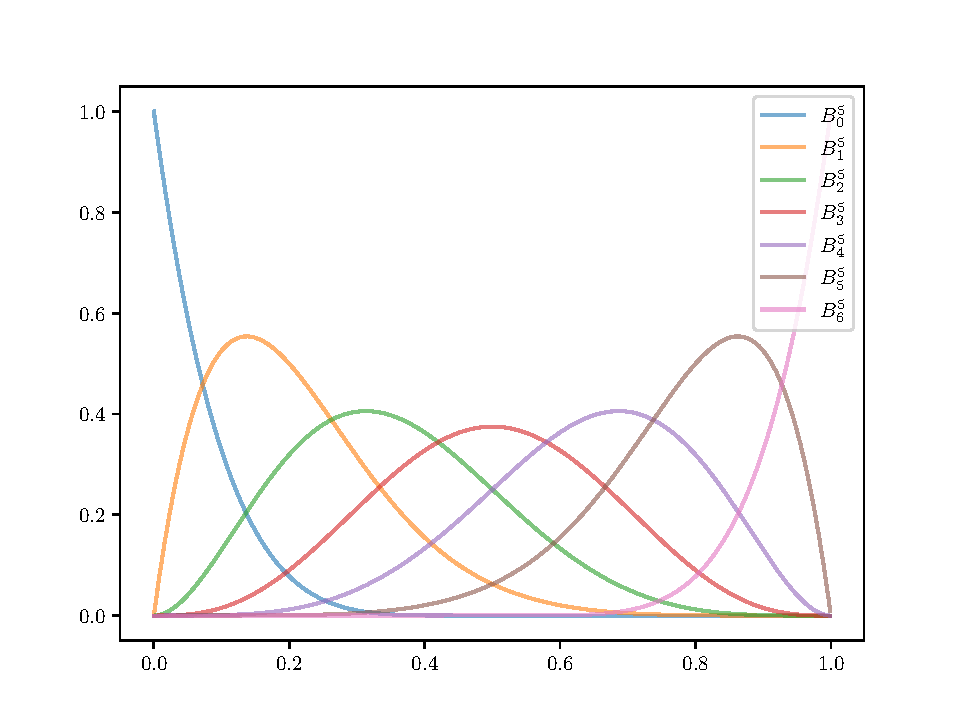
\includegraphics[width=0.8\textwidth]{Figs/AppendixA/bspline_basis.pdf}
	\caption{Example of B-spline basis functions of order $5$.}%
    \label{FIG:BSPLINE-BASIS}
\end{figure}
\begin{figure}[t]
	\centering
	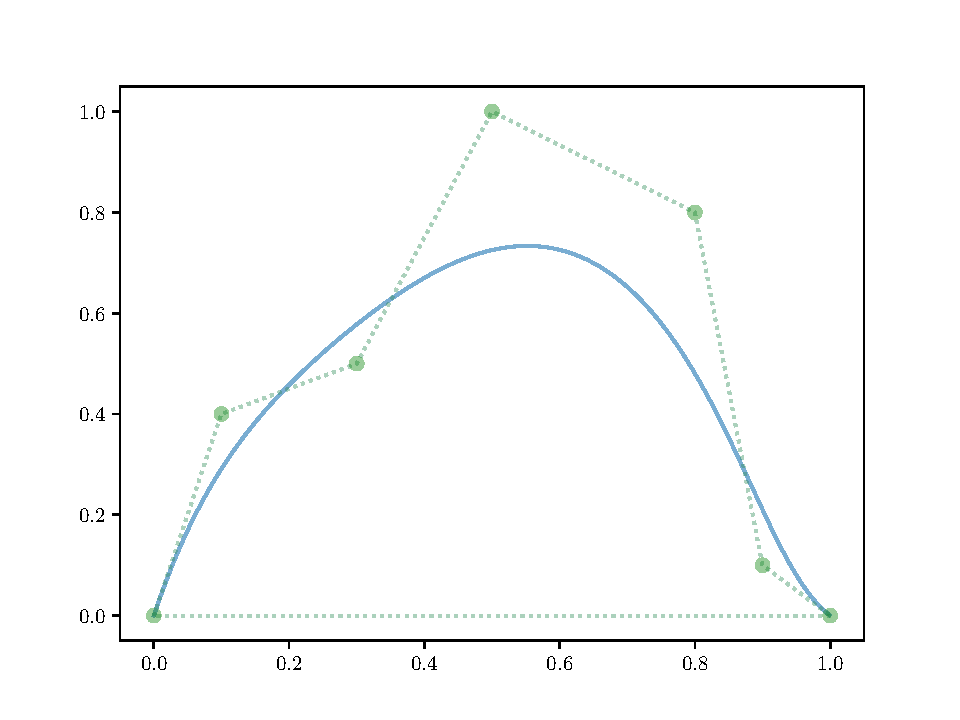
\includegraphics[width=0.8\textwidth]{Figs/AppendixA/bspline_example.pdf}
	\caption{Example of B-spline curve of order $5$.}%
    \label{FIG:BSPLINE-CURVE}
\end{figure}

%----------------------------------------------------------------------------------------
\section{NURBS Curves}
The Non Uniform Rational B-Spline (NURBS) is a generalization of the classic B-spline curves that implements a set of $\cpnumber$ additional
parameters encoded as control points \emph{weight}. A NURBS curve of order $\order$ is defined as
\begin{equation*}
    \begin{matrix}
        \bs{\spline}\lp \splinevar \rp = \frac{\sum_{i=0}^{\cpnumber} \bs{\cpoint}_{i}w_{i}\basis_{i}^{\order} \lp \splinevar \rp}
        {\sum_{i=0}^{\cpnumber} w_{i}\basis_{i}^{\order} \lp \splinevar \rp} & \text{with} & \splinevar_{\text{min}} \le \splinevar \le \splinevar_{\text{max}},
    \end{matrix}
\end{equation*}
where $\bs{\cpoint}_{i}$ is the $i$th control point, $w_{i}$ the $i$th weight and $\basis_{i}^{\order}$ the B-spline basis function.
An example of a NURBS curve of order $3$ is reported in~\figref{FIG:NURBS-CURVE}, where the weight associated with the $4$th 
control point is left free to span the range $\lp 0, 5 \rps$ while all others are fixed at $1$, note that the introduce degree
of freedom allows to locally shape the curve toward the control point just by increasing the associated weight.
In this context, the absolute value of the single weight does not play a role in the final curve shape, which instead is governed
by the value of the relative weight. As a matter of fact, if the weights are constant and equal the NURBS degenerate to a B-spline curve.
The aforementioned relation can be rewritten in B-form by setting
\begin{equation*}
    \begin{matrix}
        N_{i}^{\order} \lp \splinevar \rp = \frac{w_{i}\basis_{i}^{\order} \lp \splinevar \rp}
        {\sum_{i=0}^{\cpnumber} w_{i}\basis_{i}^{\order} \lp \splinevar \rp}
        & \implies &
        \bs{\spline} \lp \splinevar \rp = \sum_{i=0}^{\cpnumber} \bs{\cpoint}_i N_i^{\order} \lp \splinevar \rp,
    \end{matrix}
\end{equation*}
in this setting, $N_{i}^{\order}$ are piecewise rational functions, called \emph{rational basis functions}.
All properties stated for the B-splines hold also for NURBS curves with the only exception that the NURBS derivates
cannot be represented in B-form. This limits their application in motion planning due to the poor practical
derivates bounds evaluation and implementation.
\begin{figure}[t]
	\centering
	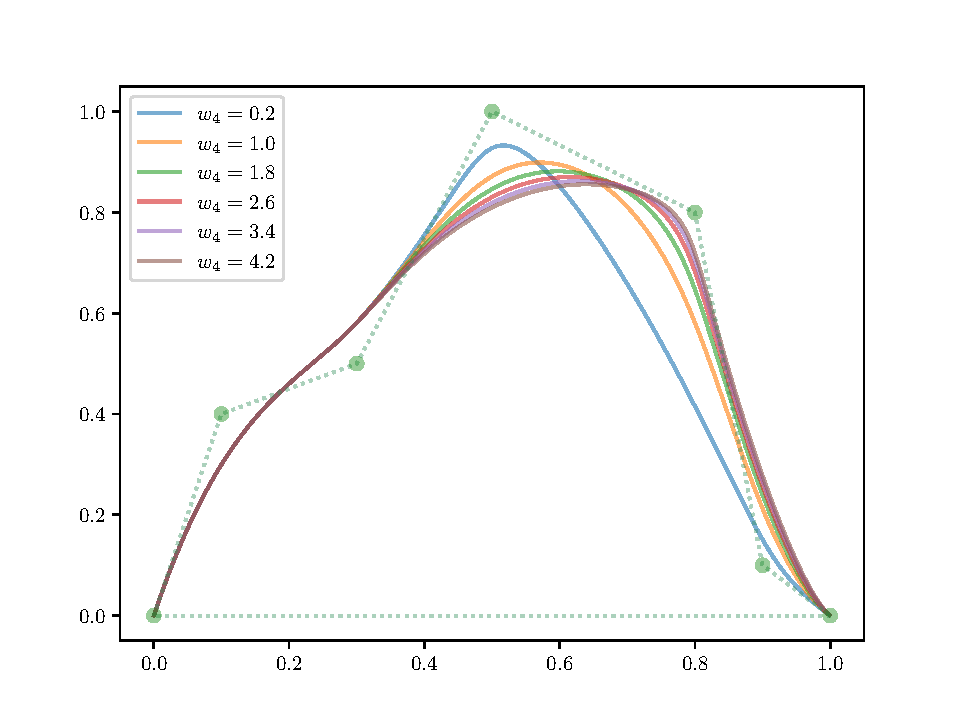
\includegraphics[width=0.8\textwidth]{Figs/AppendixA/nurbs_example.pdf}
	\caption{Example of NURBS curve of order $3$.}%
    \label{FIG:NURBS-CURVE}
\end{figure}

%----------------------------------------------------------------------------------------
\section{Relation Between B-Spline \& NURBS Curves}
Even if NURBS curves can be represented in B-form, which resembles the B-spline notation, the obtained curve is not a \emph{non-rational}
B-spline, leading to inefficient representation and evaluation, jointly with the loss of some good properties.
An efficient way to represent NURBS curves is based on homogeneous coordinates.
In the three-dimensional case, for a given set of control points $\bs{\cpoint}_i = \lps \cpoint_{x,j}, \cpoint_{y,j}, \cpoint_{z,j} \rps\T$
and weights $w_i$, it is possible to construct the weighted control points
$\bs{\cpoint}^w_i = \lps w_i\cpoint_{x,j}, w_i\cpoint_{y,j}, w_i\cpoint_{z,j}, w_i \rps\T \in \R^{4}$, which define the nonrational B-spline
\begin{equation*}
    \bs{\spline}^w(\splinevar) = \sum_{i=0}^{\cpnumber} \bs{\cpoint}^w_i \basis_i^{\order} \lp \splinevar \rp.
\end{equation*}
The latter representation and the NURBS curve formulation are equivalent in the sense that they are related to a bijective map.

%----------------------------------------------------------------------------------------
\section{B\acuteacc ezier Curves}
While NURBSs are a generalization of B-splines, B\acuteacc ezier curves represent a specialization of them.
In particular, a B\acuteacc ezier curve can be obtained from a B-spline by setting the control points number
equal to the curve order (\ie~$\cpnumber = \order$) and letting the knots vector degenerate to
\begin{equation*}
    \bs{\splinevar} = \lps \splinevar^0_{\text{min}}, \dots, \splinevar^{\order}_{\text{min}},
    \splinevar^0_{\text{max}}, \dots, \splinevar^{\order}_{\text{max}} \rps.
\end{equation*}
Usually, in this framework, the spline variable bounds are chosen as $\splinevar_{\text{min}} = 0$ and $\splinevar_{\text{max}} = 1$.
The obtained curve is still in B-form, but allows for a more efficient evaluation
\begin{equation}%
    \label{EQ:BEZIER-FORM}
    \begin{matrix}
        \bs{\spline}(\splinevar) = \sum_{i=0}^{\cpnumber} \bs{\cpoint}_i \basis_i^{\order} \lp \splinevar \rp &
        \text{with} & 0 \le \splinevar \le 1,
    \end{matrix}
\end{equation}
where the coefficients $\bs{\cpoint}_i$ are the control points, and the basis functions $\basis_i^{\order} \lp \splinevar \rp$
are $\order$th order \emph{Bernstein} polynomials defined by
\begin{equation*}
    \basis_i^{\order} \lp \splinevar \rp =
    \begin{pmatrix}
        \order \\ i
    \end{pmatrix} \splinevar^i (1-\splinevar)^{\order-i}.
\end{equation*}
In this context, the possibility to evaluate the curve without a recursive formula allows for a more efficient implementation.
The B\acuteacc ezier curves, unlike B-splines and NURBSs, enjoy a set of new properties~\cite*{farouki2012bernstein}, summarized in the following.
\begin{enumerate}
    \item \emph{Derivate}.
    The B\acuteacc ezier space is closed with respect to the operation of derivation,
    as a matter of fact, the basis function satisfies
    \begin{equation*}
        \frac{d}{d\splinevar}\basis_i^{\order} \lp \splinevar \rp =
        \order \lp \basis_{i-1}^{\order-1} \lp \splinevar \rp - \basis_{i}^{\order-1} \lp \splinevar \rp \rp,
    \end{equation*}
    that, jointly with~\eqqref{EQ:BEZIER-FORM}, yields to
    \begin{equation*}
        \frac{d}{d\splinevar}\bs{\spline}(\splinevar) =
        \sum_{i=0}^{\cpnumber-1} \order \lp \bs{\cpoint}_{i+1} - \bs{\cpoint}_{i} \rp \basis_i^{\order-1} \lp \splinevar \rp,
    \end{equation*}
    which in turn still represents a B\acuteacc ezier curve of lower degree.
    \item \emph{Arithmetic operations}. Two curves can be added, subtracted, or multiplied in a new
    B\acuteacc ezier curve by acting only on the respective control points. In particular, as regards addition and subtraction,
    the operation can be done by simply adding or subtracting the control points element-wise. If the two curves have different
    degrees, the lowest must be elevated to match the other one (see next properties). In case of product, two B\acuteacc ezier curves
    with coefficients $\bs{\cpoint}^1_0, \dots, \bs{\cpoint}^1_{\cpnumber_1}$ and $\bs{\cpoint}^2_0, \dots, \bs{\cpoint}^2_{\cpnumber_2}$,
    can be combined in a new curve with control points
    \begin{equation*}
        \bs{\cpoint}^3_i = \sum_{j = \max \lp 0, i-\cpnumber_2 \rp}^{\min \lp \cpnumber_1, i \rp}
        \frac{
            \begin{pmatrix}
                \cpnumber_1 \\ j
            \end{pmatrix}
            \begin{pmatrix}
                \cpnumber_2 \\ i-j
            \end{pmatrix}
        }{
            \begin{pmatrix}
                \cpnumber_1 + \cpnumber_2 \\ i
            \end{pmatrix}
        }
        \bs{\cpoint}^1_j \bs{\cpoint}^2_{i-j}.
    \end{equation*}
    \item \emph{Curve composition}. Two curves $\spline \lp \splinevar \rp$ and $\splinevar \lp \bar{\splinevar} \rp$ with Bernstein
    coefficients $\bs{\cpoint}^{\spline}_{0}, \dots, \bs{\cpoint}^{\spline}_{\cpnumber_{\spline}}$
    and $\cpoint^{\splinevar}_{0}, \dots, \cpoint^{\splinevar}_{\cpnumber_{\splinevar}}$ can be composed in a new B\acuteacc ezier curve
    $\bar{\spline} \lp \bar{\splinevar} \rp = \spline \lp \splinevar \lp \bar{\splinevar} \rp \rp$ via the recoursive formula
    \begin{equation*}
        \begin{split}
            \lambda_{i,j}^k =
            \begin{pmatrix}
                k \cpnumber_{\splinevar} \\ j
            \end{pmatrix}^{-1}
            \sum_{l = \max \lp 0, j - \cpnumber_{\splinevar} \rp}^{\min \lp j, k \cpnumber_{\splinevar} - \cpnumber_{\splinevar} \rp} &
            \begin{pmatrix}
                k \cpnumber_{\splinevar} - \cpnumber_u \\ l
            \end{pmatrix}
            \begin{pmatrix}
                \cpnumber_{\splinevar} \\ j-l
            \end{pmatrix} \\
            & \lps \lp 1-\cpoint^{\splinevar}_{j-l} \rp \lambda_{i,l}^{k-1} + \cpoint^{\splinevar}_{j-l}\lambda_{i+1,l}^{k-1} \rps
        \end{split}
    \end{equation*}
    for $k = 1, \dots, \cpnumber_{\spline}$, $i = 0, \dots, \cpnumber_{\spline}-k$, and $j = 0, \dots, k \cpnumber_{\splinevar}$,
    and by setting $\lambda^0_{i,0} = \bs{\cpoint}^{\spline}_i$. Finally the Bernstein coefficients of the composed curve are specified by
    \begin{equation*}
        \begin{matrix}
            \bs{\cpoint}^{\bar{\spline}}_i = \lambda_{0,j}^{\cpnumber_{\spline}}, & j = 0, \dots, \cpnumber_{\spline}\cpnumber_{\splinevar}
        \end{matrix}
    \end{equation*}
    \item \emph{Degree elevation}. A curve of order $\order$ and with coefficients $\bs{\cpoint}_0, \dots, \bs{\cpoint}_{\cpnumber}$
    can be expressed in the Bernstein basis of degree $\order + r$, for all $r > 0$, as $\bs{\spline}^{\order + r} \lp \splinevar \rp =
    \sum_{i = 0}^{\cpnumber+r} \bs{\cpoint}_i^{\order+r} \basis_{i}^{\order+r} \lp \splinevar \rp$ where the coefficients can be computed as
    \begin{equation*}
        \bs{\cpoint}_i^{\order+r} = \sum_{j = \max \lp 0, i-r \rp }^{\min \lp  \cpnumber, k \rp} \frac{
            \begin{pmatrix}
                r \\ i-j
            \end{pmatrix}
            \begin{pmatrix}
                \cpnumber \\ j
            \end{pmatrix}
        }{
            \begin{pmatrix}
                \cpnumber+r \\ i
            \end{pmatrix}
        } \bs{\cpoint}_j
    \end{equation*}
    \item \emph{Scaling the independent variable}. The change of variable $\splinevar \mapsto \lambda\splinevar$ maps the interval
    $\lps 0, 1 \rps$ to $\lps 0, \lambda \rps$, without changing the curve path, and scaling the $k$th derivate of $\lambda^{-k}$.
\end{enumerate}
The latter properties are not completely for free, as a matter of fact, the B\acuteacc eziez curve requires a higher number of parameters to
express the same spline with respect to B-splines or NURBs. On the other hand, the B\acuteacc eziez parameterization leads to a less conservative
containment property, since the obtained convex hull is tighter over the curve itself~\cite*{tordesillas2020minvo}.
Notice how going from general formulations (NURBS) to specialized forms (B-spline, B\acuteacc ezier), the number of properties increases
a lot, but loses curve flexibility and degrees of freedom.

%----------------------------------------------------------------------------------------
\section{Relation Between B-Spline \& B\acuteacc ezier Curves}
The relation linking B-spline and B\acuteacc ezier curves is purely algebraic and goes through their matrix representation.
To give an insight to the reader, both parameterizations can be represented in a form 
\begin{equation*}
   \bs{\spline} \lp \splinevar \rp =
    \begin{bmatrix}
        1 & \splinevar & \splinevar^2 & \cdots & \splinevar^{\order}
    \end{bmatrix}\T
    \bs{\basis}
    \begin{bmatrix}
        \bs{\cpoint}_0 & \bs{\cpoint}_1 & \cdots & \bs{\cpoint}_{\cpnumber}
    \end{bmatrix}\T,
\end{equation*}
with $\bs{\basis}$ being different depending on if $\bs{\spline}\lp \splinevar \rp$ represents a B-spline or a B\acuteacc ezier curve.
Let $\bs{\basis}_{\text{BS}}$ and $\bs{\basis}_{\text{BC}}$ the two matrices representing a B-spline and a B\acuteacc ezier curve,
respectively, moreover let $\bs{\cpoint}_{\text{BS}}$ and $\bs{\cpoint}_{\text{BC}}$ the associated control points, then
the following relation holds
\begin{equation*}
    \begin{bmatrix}
        \bs{\cpoint}_{\text{BS}_0} & \bs{\cpoint}_{\text{BS}_1} & \cdots & \bs{\cpoint}_{\text{BS}_{\cpnumber}}
    \end{bmatrix}\T = 
    \bs{\basis}_{\text{BS}}^{-1}
    \bs{\basis}_{\text{BC}}
    \begin{bmatrix}
        \bs{\cpoint}_{\text{BC}_0} & \bs{\cpoint}_{\text{BC}_1} & \cdots & \bs{\cpoint}_{\text{BC}_{\cpnumber}}
    \end{bmatrix}\T.
\end{equation*}
For further information about the construction of matrices $\bs{\basis}_{\text{BS}}$ and $\bs{\basis}_{\text{BC}}$, the reader is referred
to~\cite*{qin1998general}.
